\documentclass[12pt]{article}
\usepackage[utf8]{inputenc}
\usepackage[french]{babel}
\usepackage{graphicx}
\usepackage{listings}
\usepackage{float}
\usepackage{setspace}
\usepackage[colorinlistoftodos]{todonotes}

%Police
%\usepackage{helvet}
%\renewcommand{\familydefault}{\sfdefault}
%\usepackage[scaled]{arial}
%\renewcommand*\familydefault{\sfdefault} %% Only if the base font of the document is to be sans serif
\usepackage[T1]{fontenc}
\usepackage{amssymb}
\usepackage{verbatim}
\usepackage{amsmath}

% ----------------------------------
\usepackage{algorithm}
\usepackage{algorithmic}
% ----------------------------------
\renewcommand{\algorithmicensure}{\textbf{Post-conditions :}}
\renewcommand{\algorithmicend}{\textbf{fin}}
\renewcommand{\algorithmicrequire}{\textbf{Pré-conditions :}}
\renewcommand{\algorithmicif}{\textbf{si}}
\renewcommand{\algorithmicthen}{\textbf{alors}}
\renewcommand{\algorithmicelse}{\textbf{sinon}}
\renewcommand{\algorithmicelsif}{\algorithmicelse\ \algorithmicif}
\renewcommand{\algorithmicendif}{\algorithmicend\ \algorithmicif}
\renewcommand{\algorithmicfor}{\textbf{pour}}
\renewcommand{\algorithmicforall}{\textbf{pour tout}}
\renewcommand{\algorithmicdo}{\textbf{faire}}
\renewcommand{\algorithmicto}{\textbf{jusqu'à}}
\renewcommand{\algorithmicendfor}{\algorithmicend\ \algorithmicfor}
\renewcommand{\algorithmicwhile}{\textbf{tant que}}
\renewcommand{\algorithmicendwhile}{\algorithmicend\
\algorithmicwhile}
\renewcommand{\algorithmicloop}{\textbf{boucler}}
\renewcommand{\algorithmicendloop}{\algorithmicend\
\algorithmicloop}
\renewcommand{\algorithmicrepeat}{\textbf{répéter}}
\renewcommand{\algorithmicuntil}{\textbf{jusqu'à}} 

% ----------------------------------
%\everymath{\displaystyle}

\title{Cahier des charges GSI}
\begin{document}

\begin{titlepage}

\newcommand{\HRule}{\rule{\linewidth}{0.5mm}} % Defines a new command for the horizontal lines, change thickness here

\center % Center everything on the page
 
%----------------------------------------------------------------------------------------
%	HEADING SECTIONS
%----------------------------------------------------------------------------------------

\textsc{\LARGE EISTI}\\[1.2cm] % Name of your university/college
\textsc{\Large Cahier des Charges}\\[0.5cm] % Major heading such as course name
%\textsc{\large Les conférences}\\[0.5cm] % Minor heading such as course title

%----------------------------------------------------------------------------------------
%	TITLE SECTION
%----------------------------------------------------------------------------------------

\HRule \\[0.4cm]
{ \huge \bfseries Optimisation difficile pour des problème à variable continue}\\[0.4cm] % Title of your document
\HRule \\[1.5cm]
 
%----------------------------------------------------------------------------------------
%	AUTHOR SECTION
%----------------------------------------------------------------------------------------

\begin{minipage}{0.4\textwidth}
\begin{flushleft} \large
\emph{Auteurs:}\\
Elie \textsc{Poussou}
Ludovic \textsc{Lamarche}
Nicolas \textsc{Behra}
\end{flushleft}
\end{minipage}
~
\begin{minipage}{0.4\textwidth}
\begin{flushright} \large
\emph{Professeur:} \\
Rémi \textsc{Vernay} % Supervisor's Name
\end{flushright}
\end{minipage}\\[2cm]

% If you don't want a supervisor, uncomment the two lines below and remove the section above
%\Large \emph{Author:}\\
%John \textsc{Smith}\\[3cm] % Your name

%----------------------------------------------------------------------------------------
%	DATE SECTION
%----------------------------------------------------------------------------------------

{\large \today}\\[3cm] % Date, change the \today to a set date if you want to be precise

%----------------------------------------------------------------------------------------
%	LOGO SECTION
%----------------------------------------------------------------------------------------


\includegraphics[scale=.25]{EISTI.jpg}\\[1cm] % Include a department/university logo - this will require the graphicx package
 
%----------------------------------------------------------------------------------------

\vfill % Fill the rest of the page with whitespace

\end{titlepage}
\renewcommand{\contentsname}{Sommaire}
\doublespacing
\tableofcontents
\singlespacing

\newpage



\section*{Introduction}

Dans le cadre de notre 3ème semestre de cycle ingénieur, il a été proposé aux élèves du parcours GSI un projet dont le but est de créer une librairie permettant d'effectuer une optimisation difficile pour des problèmes à variable continue.

Pour mener à bien ce projet, il nous a été imposé l'utilisation de trois méta-heuristiques connues dans la recherche informatique. 

Cette librairie pourra fonctionner sur un seul ordinateur en mode séquentiel ou sur plusieurs ordinateurs en mode parallèle. 

Ce cahier des charges a pour but de proposer notre compréhension du sujet en le reformulant en clarifiant les points clefs. 

Après avoir redéfini le terme de méta-heuristiques qui sont un ensemble de solutions globales à des problèmes difficiles, nous expliquerons les trois algorithmes que nous utiliserons lors de ce projet. 

Ensuite, nous vous présenterons les technologies que nous utiliserons pour faire une solution multicœurs et multi machines. 

Enfin, nous proposerons notre planning prévisionnel qui définira la date des différents rendus intermédiaires et qui sera notre marche à suivre. 

\section{Reformulation du sujet}
	Le but du projet et de créer une librairie permettant de résoudre des problèmes complexes et d'optimisation difficile à variable continue. C'est à dire que cette API devra pouvoir résoudre n'importe quel modèle mathématique tiré d'une situation particulière. Pour cela nous allons devoir utiliser des métaheuristiques telles que l'algorithme des colonies de fourmis, d'abeilles artificielles et des essaims particulaires.
    
Dans un premier temps les algorithmes doivent s'exécuter de manière séquentielle. Ensuite nous devrons améliorer cette version en utilisant la programmation multicœurs mono-machine puis multi-machines.

   
    

\subsection{Méta-heuristique}

Le mot Méta-heuristique est composé du préfixe \textit{méta} qui signifie "dans un niveau supérieur" et de \textit{heuristique} qui vient du verbe heuriskein qui signifie "trouver". 

Étymologiquement, ce mot signifie donc trouver des solutions à des problèmes difficiles. 

Les méta-heuristiques sont un ensembles de méthodes permettant de concevoir des algorithmes afin de résoudre une large gamme de problèmes difficiles sans nécessiter de grand changement dans l'algorithme. Elles doivent pouvoir s'adapter à une large gamme de problèmes. 


Les méta-heuristiques sont généralement des méthodes stochastiques par opposition aux méthodes déterministes. En effet, ces méthodes utilisent le hasard pour éviter de parcourir l'espace de recherche en entier. 

Plus précisément, ces méthodes fournissent des stratégies pour guider à la recherche d'une solution optimale, l'espace de recherche est exploré efficacement afin de déterminer cette solution. 

Les solutions générées par les méta-heuristiques sont optimales mais ce ne sont pas les meilleures possibles, ceci étant dû à la part d'aléa.

Les méta-heuristiques sont souvent inspirées de phénomènes naturels. Dans le cadre de notre projet, nous allons  utiliser des algorithmes inspirés de l'éthologie, c'est à dire l'étude du comportement des espèces animales dans leur milieu naturel. 

Nous allons détailler dans les prochaines parties chaque algorithme utilisé. 



\subsection{Colonies de fourmis \cite{fourmis}}
%http://www.eyrolles.com/Chapitres/9782212113686/chap4_Dreo.pdf

L'algorithme des colonies de fourmis est une métaheuristique récente qui s'inspire de l'auto-organisation dans le monde des insectes. Cette une technique est le fait de faire communiquer une colonie d'individus (ici les fourmis) en modifiant leur environnement. Le but est de comprendre ce phénomène biologique et de le comparer à des problèmes tels que celui du voyageur de commerce pour ensuite proposer un algorithme permettant d'optimiser la solution du problème.

\subsubsection{Optimisation naturelle: piste des phéromones}
	Les biologistes ont constaté que les colonies de fourmis et les insectes sociaux résolvent naturellement des problèmes complexes. Ces problèmes sont impossibles à résoudre pour un seul individu, par exemple le choix de l'exploitation des sources de nourriture. Pour communiquer, les fourmis utilisent ce qu'on appelle des phéromones. Elles en déposent au sol lorsqu'elles se déplacent. Ainsi les fourmis créent des pistes que les autres peuvent suivre.
    
    Lorsqu'une fourmi repère une source de nourriture, quelques-unes s'y rendent sans connaître le meilleur chemin et retournent à leur fourmilière. Ensuite les fourmis suivantes vont suivre la piste qui a le plus de phéromones. En fait plus le trajet est long, plus les phéromones auront eu le temps de s'évaporer. Ainsi les fourmis suivantes choisissent naturellement le chemin le plus cours.
    
\begin{figure}[H]
	\centering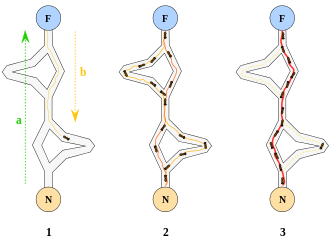
\includegraphics[scale=1]{pisteFourmis.png}
    \caption{Résolution du chemin le plus court par les fourmis}
\end{figure}	



\subsubsection{Voyageur de commerce}
Le premier algorithme permettant d'optimiser le problème du voyageur de commerce est celui de l'Ant System. Nous allons détailler cette première approche pour mieux comprendre le fonctionnement d'une colonie de fourmis pour résoudre le voyageur de commerce.

L'objectif du voyageur de commerce est de trouver un parcours dans un graphe qui passe par tous les nœuds une seule et unique fois et dont le coût (ici la distance) est minimal.

L'algorithme se déroule à un instant $t$ ($1<t<t_{max}$) où chaque fourmis $k$ parcourt un nœud du graphe. Soit $i$ le nœud courant et $j$ le nœud suivant. Le choix du nœud suivant dépend de plusieurs critères :
\begin{itemize}
\item La liste des nœud déjà visités par la fourmi $k$ : $J^k_i$.
\item L'inverse de la distance entre le nœud courant et les suivants noté $n_{ij}=\frac{1}{d_{ij}}$
\item La quantité de phéromone se trouvant sur l'arête entre $i$ et $j$. Cette quantité évolue en fonction du temps et du nombre de passages de fourmis.

\end{itemize}

La règle de déplacement donnée par Bonabeau\cite{fourmis} est la suivante :
\[
p^k_{ij}(t) = 
\left\{\begin{array}{cc}
\frac{\Gamma_{ij}(t)^\alpha . n_{ij}^\beta}{\sum_{l\in J^k_i} (\Gamma_{il}(t)^\alpha . n_{ij}^\beta)} &
\textnormal{si }j\in J_i^k \\
0 & \textnormal{si }j\notin J_i^k
\end{array}
\right.
\]

$\alpha$ contrôle l'intensité de la piste $\Gamma_{ij}(t)$ et $\beta$ contrôle la visibilité.

À la fin de son parcours, la fourmi laisse une certaine quantité de phéromones sur son trajet. Cette quantité est définie par l'expression suivante:
\[
\Delta\Gamma^k_{ij}(t) = 
\left\{\begin{array}{cc}
\frac{Q}{L^k(t)} &
\textnormal{si }(i,j)\in T^k(t) \\
0 & \textnormal{si }(i,j)\notin T^k(t)
\end{array}
\right.
\]

$T^k(t)$ et le parcours de la fourmi $k$ à l'instant $t$, $L^k(t)$ la longueur du tour et $Q$ un paramètre fixé.

Enfin il faut prendre en compte l'évaporation des phéromones avec une autre fonction. Pour cela nous allons diminuer à chaque instant la valeur des arêtes du graphe grâce à la fonction suivante :
$$
\Gamma_{ij}(t+1) = (1-p).\Gamma_{ij}(t) + \Delta\Gamma_{ij}(t)
$$
Où $\Delta_{ij}(t)$ est la quantité de phéromones déposé par toute les fourmis.

\newpage
\subsubsection{Algorithme}

\begin{algorithm}
    \caption{Algorithme de colonies de fourmis de base : "Ant System"}
    \begin{algorithmic}
    %%-----------------------------------------------
          \FOR{$ t = 1 $ \TO $t_{max}$ }
          	\FOR{ chaque fourmis $ k = 1 $ \TO $m$ }
            \STATE{Choisir un nœud au hasard}
            \FOR{ chaque nœud $i$ non visité}
             \STATE{Choisir un nœud $j$ dans la liste $J^k_i$ des nœuds restants selon la formule vue précédemment} 
            \ENDFOR
            \STATE{Ajouter la piste $\Delta\Gamma^k_{ij}(t)$ sur le trajet $T^k(t)$}
          \ENDFOR
          \STATE{Évaporer les phéromones}
      	\ENDFOR
    %%-----------------------------------------------
    \end{algorithmic}
    \end{algorithm}




\subsection{Colonies d'abeilles artificielle \cite{abeilles}}
%https://msdn.microsoft.com/fr-fr/magazine/gg983491.aspx
 L'abeille est un des insectes les plus organisés et les plus rigoureux dans leur travail. Les abeilles possèdent une très grande capacité de communication grâce notamment à des danses. Dans cette méthode, les abeilles représentent des agents qui, en collaborant les unes avec les autres, résolvent des problèmes complexes d'optimisation combinatoire.
 
\subsubsection{Présentation du phénomène naturel}
Une ruche contient de 5000 à 20000 abeilles. Les abeilles adultes deviennent généralement des butineuses. 
Ces butineuses sont environ réparties de la manière suivante : 
\begin{itemize}
   \item 75\% d'actives qui volent jusqu'à la source de nourriture, explorent les sources de nourriture voisines, recueillent la nourriture et reviennent à la ruche.
   \item 10\% d'inactives qui attendent à la ruche et qui peuvent relayer les actives. 
   \item 15\% d'éclaireuses qui cherchent de nouvelles sources de nourriture attirantes. 
\end{itemize}

À leur retour à la ruche, les éclaireuses et butineuses font une danse qui donne des informations sur la localisation et la qualité de la nourriture. 

Les abeilles inactives deviennent actives et suivent les informations fournies précédemment par les danses. 

Au fur et à mesure, la qualité de la nourriture trouvée est optimisée puisque chaque abeille qui va recueillir de la nourriture cherche des nouvelles sources de nourriture. Chaque nouvelle source est évaluée par les abeilles 
\subsubsection{Paramètres et fonctions nécessaires à l'implémentation}

L'algorithme qui s'inspire de ce phénomène peut servir à résoudre des problèmes combinatoires complexes comme par exemple le voyageur de commerce. 

L'algorithme part d'une solution initiale aléatoire et tend à l'améliorer, les abeilles représentent les agents qui permettent l'amélioration de la solution.

A l'initialisation, un ensemble d'abeilles est créé, chacune dispose d'une solution aléatoire. 

Chaque abeille dispose des attributs suivants :
\begin{itemize}
	\item Le statut (active, inactive ou éclaireuse)
    \item Une matrice en mémoire qui représente une solution trouvée par cette abeille. 
    \item Une mesure de la qualité de la solution, cette mesure est calculée à partir de la matrice précédente. 
    \item Un nombre de visites maximum : si l'abeille revient sur la même solution plus de fois que le nombre de visites maximum, l'abeille devient inactive et une autre abeille inactive devient active. 
    \item 
\end{itemize}
Chaque implémentation de l'algorithme des colonies d'abeilles doit avoir :
\begin{itemize}
\item Une fonction qui génère une solution aléatoire. 
\item Une fonction de mesure de la qualité d'une solution. Par exemple, dans le cas du problème du voyageur de commerce, cette fonction calculerait le coût du chemin final. 
\item Une fonction qui génère une solution voisine à partir d'une solution apportée par une abeille. Grâce à cette nouvelle solution voisine générée, l'abeille pourra parcourir le voisinage d'une solution déjà bonne pour essayer d'en trouver une encore meilleure. 
\end{itemize}

\subsubsection{Déroulement de l'algorithme}

Pour détailler le déroulement de cet algorithme, nous allons séparer le comportement de chaque type d'abeille. 
\begin{itemize}
\item \emph{ Les abeilles actives } : Chaque abeille active a une solution aléatoire à l'initialisation. 

Une solution voisine est générée à partir de cette solution, cette solution voisine est évaluée par la fonction qui évalue la qualité d'une solution. 

Si cette solution est meilleure que la précédente, l'abeille met à jour sa solution en mémoire et une autre solution voisine est générée et  on recommence l'étape précédente. 
Si la solution n'est pas meilleure, un compteur est incrémenté et une nouvelle solution voisine est générée.  

Tant que le compteur ne dépasse pas la limite du nombre maximal de visites, on recommence les opérations précédentes. 

L'abeille active passe à l'état inactif lorsque le compteur dépasse cette limite. Cela signifiera qu'il n'aura pas trouvé de solution voisine meilleure que la solution courante après un grand nombre d'essais. 

Lors de son passage à l'état inactif, si la nouvelle solution de cette abeille est meilleure que la solution globale, cette solution globale est mise à jour et des informations sur cette nouvelle solution sont transmises aux abeilles inactives. 

\item \emph{ Les abeilles inactives} : Dès qu'une abeille active passe à l'état inactif, une abeille inactive tirée aléatoirement prend sa place en copiant en mémoire les informations transmises par l'abeille active.

\item \emph{Les abeilles éclaireuses} : Elles génèrent des solutions aléatoires en espérant en trouver une meilleure que la solution globale. 


\end{itemize}

\subsection{Essaims particulaires \cite{essaim1} }

    En étudiant le comportement d'un groupement d'animaux tel que des vols d'oiseaux ou des bancs de poissons, on observe que le déplacement d'un individu détermine le déplacement des autres. On a ici le concept d'auto-organisation comme les colonies de fourmis. 

    \begin{figure}[H]
        \centering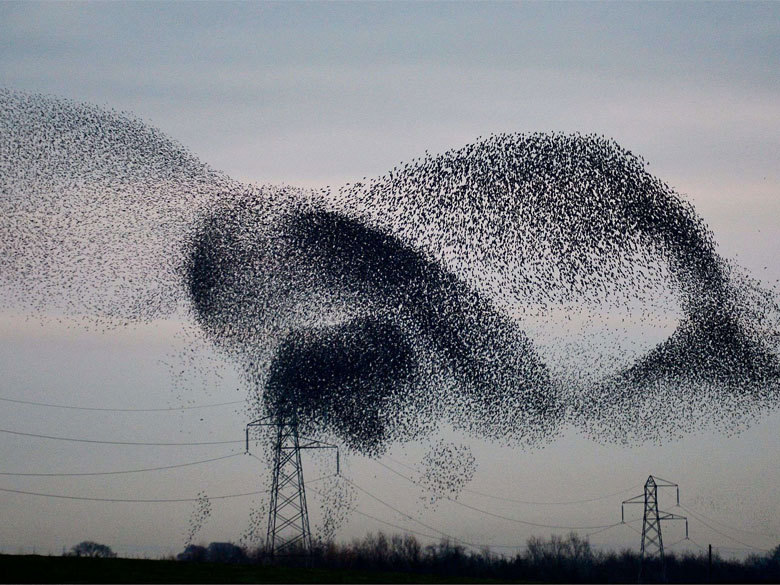
\includegraphics[scale=0.4]{vol-groupe-d-oiseaux.jpg}
        \caption{Vol d'oiseaux en Ecosse}
    \end{figure}	

    “L'union fait la force” voila la seule règle d'or quant à la survie dans le monde du vivant concernant les espèces d'animaux se déplaçant en groupe, ceci signifie qu'un individu de ce groupe pris à part est évalué comme peu intelligent alors qu'en se regroupant il se créé une complexité et donc une intelligence. À partir des mouvements locaux de chaque individu on a un mouvement global tout en conservant une distance optimale entre chacun d'eux. Le concept d'essaim particulaire permet de déterminer l'optimum d'une fonction non-linéaire et la résolution des réseaux de neurones.

	\subsubsection{Principe de la Méthode}
    Chaque individu du groupe est considéré comme étant une particule avec une mémoire contenant des informations sur les positions optimales visitées et sur ses voisins (et peut interagir avec eux). Donc son déplacement s'effectuera en fonction d'une part de ses connaissances et d'autre part de celui de ses voisins. Ainsi l'optimum global sera déterminé grâce aux optimums locaux et empiriques de chaque individu.

	\subsubsection{Algorithme simpliste (sans voisinage) }
    Différents paramètres permettent de définir un essaim de particule tel que la vitesse maximale, la taille et la topologie du voisinage, des coefficients de confiance (qui permettent de savoir si l'individu en question doit ou pas suivre la conformité, i.e. suivre le voisin), l'inertie d'un individu et le nombre de particules constituant l'essaim.\\ \\
    \indent Cet algorithme permet de déterminer toutes les positions des particules permettant d'avoir une solution optimale globale avec:
   
\begin{itemize}
	\item \textit{ $x_{i}$ } : la position de cette particule dans l'espace;
	\item \textit{ $v_{i}$ } : sa vitesse;
	\item  \textit{ $x_{p_{i}}$ } : position par laquelle elle est déjà passée et dont la solution est la meilleure; 
	\item  \textit{ $x_{v_{i}}$ } : position du voisin pour laquelle la solution est la meilleure; 
 	\item \textit{ $F(x_{i})$ } : fonction qui détermine la valeur de convenance ou d'aptitude en fonction d'une position donnée $x$;
    \item \textit{ $\rho$ } : constante de confiance comprise entre 0 et 1;
    \item \textit{ $c_{i}$ } : la valeur de convenance ou d'aptitude correspondant à sa meilleure solution;
    \item \textit{ $c_{v_{i}}$ } : la valeur de convenance ou d'aptitude correspondant à la meilleure solution trouvée parmi son voisinage;
    \item \textit{ $nb$ } : le nombre de particules;
\end{itemize}
%% \vspace{9\baselineskip}
    \begin{algorithm}
    \caption{Algorithme Simpliste (sans voisinage)}
    \begin{algorithmic}
    %%-----------------------------------------------
      \REQUIRE $ 0 < \rho < 1 $        % demande le paq. amssymb
      \ENSURE déplacement de l'ensemble des particules
      \REPEAT
          \FOR{$ i = 1 $ \TO $nb$ }
              \IF{$ F(x_{i}) > c_{i} $} 
                  \STATE{$ c_{i} \leftarrow F(x_{i}) $}
                  \STATE{$ x_{p_{i}} \leftarrow x_{i} $}
              \ENDIF
              \STATE $ v_{i} \leftarrow v_{i} + \rho(x_{p_{i}} - x_{i}) $
              \STATE $ x_{i} \leftarrow x_{i} + v_{i} $
          \ENDFOR
      \UNTIL{ (au moins un des critères d'arrêt est atteint) }
    %%-----------------------------------------------
    \end{algorithmic}
    \end{algorithm}
    
    \subsubsection{ Détermination des paramètres }
    En ce qui concerne le \textit{nombre de particule} à choisir il faut prendre en compte l'espace de recherche, la capacité de la machine et le temps de recherche maximal acceptable. Pour ce paramètre il conviendra de faire des tests pour déterminer la valeur la plus adaptée aux trois conditions énoncées précédemment. \\
    \indent Pour les relations ou liaisons entre une particule et ses voisins, plusieurs configurations ou topologies son envisageable:
    \begin{description}
    	\item[a)] topologie en \textbf{anneau}: chaque particule communique avec n autres particules;
        \item[b)] topologie en \textbf{rayon}: toutes les particules communiquent avec une seule particule centrale;
        \item[c)] topologie en \textbf{étoile}: toutes les particules communiquent avec toutes les autres.
    \end{description}
    \begin{figure}[H]
        \centering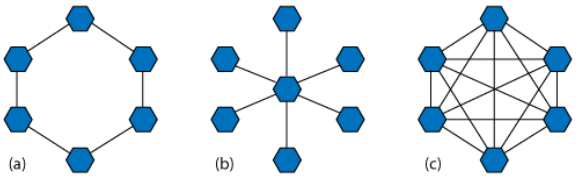
\includegraphics[scale=0.4]{topologies.png}
        \caption{ (a) anneau (n=2), (b) rayon, (c) étoile.}
    \end{figure}
    \indent La configuration en étoile n'est pas optimale car l'optimum global trouvé n'est qu'en fait un optimum local, et donc on observe une stagnation; pour palier se problème la configuration en anneau est plus lente mais plus efficace quant à la détermination d'un optimum global. Il faut trouver la topologie qui représente au mieux le phénomène observé. Si les individus de la colonie sont répartis de façon éparse, on pourra supposer que l'information mettra plus de temps à se propager, ce qui se caractérisera par une topologie contenant peu de liaison entre les individus (exemple: topologie en anneau avec $n$ petit); ou à l'inverse si les individus semblent être serrés ou former une masse compacte, alors on optera pour une topologie contenant beaucoup de liaison et donc l'information circulera beaucoup plus rapidement (exemple: topologie en rayon) \cite{essaim2}. \\
    \indent La question de la synchronisation se pose aussi. Est-ce que les individus échangent de manière synchrone,c'est à dire tous au même moment à chaque toc l'horloge, ou bien de manière asynchrone c'est à dire qu'après une ou plusieurs conditions remplient (à définir)  l'individu transmet les informations? \\
    \indent En ce qui concerne les \textit{coefficients de confiance} $\rho_{1}$ et $\rho_{2}$, ils permettent d'indiquer la tendance d'un individu à suivre son instinct ou bien à suivre une certaine conformité par rapport à l'observation de ses voisins. Ce sont deux variables aléatoires définies comme suit:
   \[
    \left\{\begin{array}{cc}
      \rho_{1} = r_{1}*c_{1} \\
      \rho_{2} = r_{2}*c_{2} 
    \end{array}
    \right.
  \]
    
Où $c_{1}$, $c_{2}$  sont deux constantes positives déterminées de façon empirique et telles que $c_{1} + c_{2} \le 4 $ et $r_{1}, r_{2}$ suivent une loi uniforme sur [0..1]. \\

Concernant la vitesse, il peut s'avérer judicieux d'imposer une vitesse maximale  pour ne pas que les individus ne se déplacent trop vite et ainsi ne pas manquer une solution optimale. On peut toute fois s'en passer en utilisant un coefficient dit de \textit{constriction}, qui permet de réduire l'espace de recherche, ce qui donne une nouvelle équation pour la vitesse: \\

$ v_{i}(t) = \kappa (v_{i}(t-1) + \rho_{1} (x_{p_{i}} - x_{i}(t)) + \rho_{2} (x_{v_{i}} - x_{i}(t))$ \\

avec $ \kappa = 1 - \frac{1}{\rho} + \frac{\sqrt{ |\rho^2 - 4\rho|}}{2} $
    et $\rho = \rho_{1} + \rho_{2} > 4$ \\ \\
    
    Grâce à ce coefficient de constriction, le taux de convergence vers une solution optimale est nettement plus élevé.
    
    Ce coefficient $\kappa$ peut être vu différemment. Vu comme un facteur d'inertie c'est à dire la faculté d'exploration des particules, plus $\kappa$ est élevé ( >1 ) plus la particule peut se mouvoir ( i.e. plus l'optimum est global) et inversement pour $\kappa$ <1. Pour espérer une meilleure convergence ce facteur doit être compris entre $0.8$ et $1.2$ .\\
    
    Concernant la position et la vitesse initiale des individus il suffit de les initialiser de manière aléatoire suivant une loi uniforme sur $[0..1]$.
    Enfin les critères d'arrêts sont les suivants (au moins un d'entre eux doit être atteint pour que l'algorithme s'arrête):

\begin{itemize}
	\item le nombre d'itération maximal ( fixé au-préalable et déterminer de manière empirique);
    \item la vitesse varie très peu (taux de variation proche de 0);
    \item l'aptitude/convenance de la solution est acceptable.
\end{itemize}
    
    
    \subsubsection{ Algorithme simpliste (avec voisinage) }
    
    \begin{algorithm}
    \caption{Algorithme Simpliste (avec voisinage)}
    \begin{algorithmic}
    %%-----------------------------------------------
      \REQUIRE $ 0 < \rho < 1 $        % demande le paq. amssymb
      \ENSURE déplacement de l'ensemble des particules
      \REPEAT
          \FOR{$ i = 1 $ \TO $nb$ }
              \IF{$ F(x_{i}) > c_{i} $} 
                  \STATE{$ c_{i} \leftarrow F(x_{i}) $}
                  \STATE{$ x_{p_{i}} \leftarrow x_{i} $}
              \ENDIF
              \IF{$ F(x_{i}) > c_{v_{i}} $} 
                  \STATE{$ c_{v_{i}} \leftarrow F(x_{i}) $}
                  \STATE{$ x_{v_{i}} \leftarrow x_{i} $}
              \ENDIF
           \ENDFOR
           \FOR{$ i = 1 $ \TO $nb$ }
              \STATE $ v_{i} \leftarrow \kappa (v_{i} + \rho_{1} (x_{p_{i}} - x_{i}) + \rho_{2} (x_{v_{i}} - x_{i}) $
              \STATE $ x_{i} \leftarrow x_{i} + v_{i} $
          \ENDFOR
      \UNTIL{ (au moins un des critères de d'arrêt est atteint) }
    %%-----------------------------------------------
    \end{algorithmic}
    \end{algorithm}
    
\section{Ressources}

\subsection{Logiciels}
Pour développer notre API en C++ nous avons à disposition deux interfaces permettant de créer des programmes muticoeurs et multi machine.


\subsubsection{MPI}
MPI\cite{mpi} (Message Passing Interface) est une librairie permettant de transmettre des messages entre différents processus. Nous nous servirons de cette API pour développer la partie multicœur.

\subsubsection{OpenMP}
OpenMP est une librairie permettant de faire des calculs parallèles entre plusieurs machines. On peut l'utiliser en C++ sur linux ou windows.

\subsection{Planning et stratégie}
\begin{tabular}{|c|c|c|}
\hline
Deadline & Missions & Développeurs \\
\hline
25/01/2015 & Définition du cahier des charges. & Elie, Ludovic, Nicolas\\
\hline
 & Algorithme des abeilles & Elie\\
08/03/2015 & Algorithme des fourmis & Ludovic\\
 & Algorithme des essaims particulaires & Nicolas\\
\hline
05/04/2015 & Implémentation multi-coeurs & Elie\\
 & Implémentation multi-machine & Ludovic, Nicolas\\
 \hline
\end{tabular}
\\\\
Nous allons donc commencer par implémenter les algorithmes cités précédemment de manière séquentielle puis nous les amélioreront en utilisant le multi-coeur et le multi-machine.

\section*{Conclusion}

L'observation des comportements animaliers, l'éthologie, est une source d'inspiration infini, quant à la réalisation d'algorithme utile à la résolution de problèmes, tel que le voyageur du commerce, la détermination d'un optimum d'une fonction non-linéaire ou encore les réseaux de neurones. Dans notre cas, le comportement des colonies de fourmis, les colonies d'abeilles et les vols d'oiseaux peut être implémenter sous condition de bien définir les paramètres d'une part et de déterminer leurs valeurs d'initialisation d'autre part, très souvent de manière empirique. Toute fois il subsiste un problème, le temps d'attente quant à la résolution d'une solution optimale est souvent très longue, c'est pourquoi après avoir implémenter ces algorithmes de mimétismes, nous les ferons tourner d'abord sur multi-coeurs puis sur plusieurs machines fonctionnant en parallèle en utilisant les technologies MPI et OpenMP dans le langage C++, pour avoir un temps d'attente moindre, une solution globale plus optimale et un nombre d'individu de départ plus élevé. Ainsi nous arriverons peut-être à résoudre l'éternelle question: qui de l'homme ou de l'animal est le plus intelligent? 



\nocite{*}
\bibliographystyle{unsrt}
\bibliography{biblio}

\end{document}